\subsection{相似多边形}\label{subsec:czjh2-6-10}
\begin{enhancedline}

前面,我们研究了相似三角形,现在来研究相似多边形。

如果两个边数相同的多边形的对应角都相等,对应边都成比例,这两个多边形叫做\zhongdian{相似多边形}。

例如,四边形 $ABCD$ 与四边形 $A'B'C'D'$ 中(图 \ref{fig:czjh2-6-34}),
\begin{align*}
    & \angle A = \angle A' \douhao \angle B = \angle B' \douhao \\
    & \angle C = \angle C' \douhao \angle D = \angle D' \fenhao \\
    & \dfrac{AB}{A'B'} = \dfrac{BC}{B'C'} = \dfrac{CD}{C'D'} = \dfrac{DA}{D'A'} = \exdfrac{2}{3} \juhao
\end{align*}

所以四边形 $ABCD \xiangsi$ 四边形 $A'B'C'D'$。 % 所以$\text{四边形} ABCD \xiangsi \text{四边形} A'B'C'D'$。

\begin{figure}[htbp]
    \centering
    \begin{minipage}[b]{7cm}
        \centering
        \begin{tikzpicture}
    \begin{scope}
        \tkzDefPoints{0/0/A, 2/0/B, 1.8/1/C, 0.8/1.5/D}
        \tkzDrawPolygon(A,B,C,D)
        \tkzLabelPoints[above](D)
        \tkzLabelPoints[right](C)
        \tkzLabelPoints[below](A,B)
    \end{scope}

    \begin{scope}[xshift=3cm,scale=1.5]
        \tkzDefPoints{0/0/A', 2/0/B', 1.8/1/C', 0.8/1.5/D'}
        \tkzDrawPolygon(A',B',C',D')
        \tkzLabelPoints[above](D')
        \tkzLabelPoints[right](C')
        \tkzLabelPoints[below](A',B')
    \end{scope}
\end{tikzpicture}


        \caption{}\label{fig:czjh2-6-34}
    \end{minipage}
    \qquad
    \begin{minipage}[b]{7cm}
        \centering
        \begin{tikzpicture}
    \begin{scope}[scale=1.5]
        \tkzDefPoints{-1/0/A, 1/0/B, 0.6/1.3/C, -0.6/1/D}
        \tkzDrawPolygon(A,B,C,D)
        \tkzLabelPoints[left](D)
        \tkzLabelPoints[right](C)
        \tkzLabelPoints[below](A,B)
    \end{scope}

    \begin{scope}[xshift=3.6cm]
        \tkzDefPoints{1/0/A', -1/0/B', -0.6/1.3/C', 0.6/1/D'}
        \tkzDrawPolygon(A',B',C',D')
        \tkzLabelPoints[right](D')
        \tkzLabelPoints[left](C')
        \tkzLabelPoints[below](A',B')
    \end{scope}
\end{tikzpicture}


        \caption{}\label{fig:czjh2-6-35}
    \end{minipage}
\end{figure}

相似多边形的对应边的比叫做\zhongdian{相似比}(或\zhongdian{相似系数})。
如图 \ref{fig:czjh2-6-35} 中的四边形 $ABCD \xiangsi A'B'C'D'$,对应边的比是 $\exdfrac{3}{2}$,
那么四边形 $ABCD$ 和 $A'B'C'D'$ 的相似比是 $k_1 = \exdfrac{3}{2}$,
  而四边形 $A'B'C'D'$ 和 $ABCD$ 的相似比是 $k_2 = \exdfrac{2}{3}$。

现在,我们来研究相似多边形的性质。

我们知道,过多边形的一个顶点的对角线有 $n - 3$ 条,它将多边形分成 $n - 2$ 个三角形,
由于我们已经学过相似三角形的性质,因此,我们先研究两个相似多边形的对应对角线的性质,
然后再利用相似三角形来研究相似多边形。

六边形 $ABCDEF \xiangsi$ 六边形 $A'B'C'D'E'F'$ % $\text{六边形} ABCDEF \xiangsi \text{六边形} A'B'C'D'E'F'$
(图\ref{fig:czjh2-6-36}),相似比为 $k$。
$AC$ 与 $A'C'$, $AD$ 与 $A'D'$, $AE$ 与 $A'E'$ 分别是对应对角线。

\begin{figure}[htbp]
    \centering
    \begin{tikzpicture}
    \def\drawingcode#1#2#3#4#5#6{
        %\tkzDrawPolygon(A,B,C,D,E)
        %\tkzDrawSegments[dashed](A,C A,D A,E)
        \tkzDrawPolygon(#1,#2,#3,#4,#5,#6)
        \tkzDrawSegments[dashed](#1,#3 #1,#4 #1,#5)
        \tkzLabelPoints[left](#1,#5,#6)
        \tkzLabelPoints[right](#2,#3)
        \tkzLabelPoints[above](#4)
    }

    \begin{scope}[scale=1.3]
        \tkzDefPoints{0/0/A, 2/0/B, 2/1.5/C, 0.8/2/D, -0.2/1.3/E, -0.4/0.6/F}
        \drawingcode{A}{B}{C}{D}{E}{F}
    \end{scope}

    \begin{scope}[xshift=4cm,scale=0.8]
        \tkzDefPoints{0/0/A', 2/0/B', 2/1.5/C', 0.8/2/D', -0.2/1.3/E', -0.4/0.6/F'}
        \drawingcode{A'}{B'}{C'}{D'}{E'}{F'}
    \end{scope}
\end{tikzpicture}


    \caption{}\label{fig:czjh2-6-36}
\end{figure}

六边形 $ABCDEF \xiangsi$ 六边形 $A'B'C'D'E'F'$

\qquad $\tuichu \left\{\begin{aligned}
    \angle B = \angle B' \\
    \dfrac{AB}{A'B'} = \dfrac{BC}{B'C'} = k
\end{aligned}\right\}  \tuichu \triangle ABC \xiangsi \triangle A'B'C'$


% \begin{wrapfigure}[6]{r}{7.4cm}
%     \centering
%     \begin{tikzpicture}
    \def\drawingcode#1#2#3#4#5#6{
        %\tkzDrawPolygon(A,B,C,D,E)
        %\tkzDrawSegments[dashed](A,C A,D A,E)
        \tkzDrawPolygon(#1,#2,#3,#4,#5,#6)
        \tkzDrawSegments[dashed](#1,#3 #1,#4 #1,#5)
        \tkzLabelPoints[left](#1,#5,#6)
        \tkzLabelPoints[right](#2,#3)
        \tkzLabelPoints[above](#4)
    }

    \begin{scope}[scale=1.3]
        \tkzDefPoints{0/0/A, 2/0/B, 2/1.5/C, 0.8/2/D, -0.2/1.3/E, -0.4/0.6/F}
        \drawingcode{A}{B}{C}{D}{E}{F}
    \end{scope}

    \begin{scope}[xshift=4cm,scale=0.8]
        \tkzDefPoints{0/0/A', 2/0/B', 2/1.5/C', 0.8/2/D', -0.2/1.3/E', -0.4/0.6/F'}
        \drawingcode{A'}{B'}{C'}{D'}{E'}{F'}
    \end{scope}
\end{tikzpicture}


%     \caption{}\label{fig:czjh2-6-36}
% \end{wrapfigure}

\qquad $\tuichu  \left\{\begin{aligned}
    & \dfrac{AC}{A'C'} = k \douhao \\
    & \angle ACB = \angle A'C'B' \juhao
\end{aligned}\right.$

由此,又可推出 $\angle ACD = \angle A'C'D'$, $\dfrac{AC}{A'C'} = \dfrac{DC}{D'C'} = k$。可得到
$$ \triangle ACD \xiangsi \triangle A'C'D'  \tuichu \dfrac{AD}{A'D'} = k \juhao $$

同理可得 $\dfrac{AE}{A'E'} = k$。

一般地,可以得到

\begin{xingzhi}
    两个相似多边形对应对角线的比等于相似比。
\end{xingzhi}

以两个相似多边形的对应顶点为顶点的两个三角形(相似多边形中的对应三角形),
它们的边或是多边形的边,或是多边形的对应对角线,所以这样的两个三角形的三边对应成比例,
它们是相似三角形。例如 $\triangle ACD \xiangsi \triangle A'C'D'$。于是有

\begin{dingli}[定理]
    相似多边形中的对应三角形相似,相似比等于相似多边形的相似比。
\end{dingli}

和相似三角形一样,利用等比定理可得:

\begin{dingli}[定理]
    相似多边形周长的比等于相似比。
\end{dingli}

我们知道,经过 $n$ 边形的任何一个顶点的 $n-3$ 条对角线,将多边形分成 $n-2$ 个环绕着这个顶点按顺序排列的三角形。
两个相似 $n$ 边形分别被这样一组对应对角线分成的对应三角形分别相似。由等比定理可得:

\begin{dingli}[定理]
    相似多边形的面积比等于相似比的平方。
\end{dingli}


\liti 四边形 $ABCD \xiangsi$ 四边形 $A'B'C'D'$,
它们的对角线分别交于点 $O$、$O'$(图 \ref{fig:czjh2-6-37})。
求证: $\triangle OAB \xiangsi \triangle O'A'B'$。

\zhengming 四边形 $ABCD \xiangsi$ 四边形 $A'B'C'D'$

\qquad $\tuichu \left\{\begin{aligned}
    \triangle ABD \xiangsi \triangle A'B'D'  \tuichu \angle 2 = \angle 4 \\
    \triangle ABC \xiangsi \triangle A'B'C'  \tuichu \angle 1 = \angle 3
\end{aligned}\right\}$

\qquad $\tuichu \triangle OAB \xiangsi \triangle O'A'B'$。

\begin{figure}[htbp]
    \centering
    \begin{minipage}[b]{7cm}
        \centering
        \begin{tikzpicture}
    \def\drawingcode#1#2#3#4{
        \tkzDrawPolygon(#1,#2,#3,#4)
        \tkzDrawSegments(#1,#3 #2,#4)
        \tkzInterLL(#1,#3)(#2,#4)  \tkzGetPoint{O}
        \tkzLabelPoints[left](#4)
        \tkzLabelPoints[right](#3)
        \tkzLabelPoints[below](#1,#2)
    }

    \begin{scope}
        \tkzDefPoints{0/0/A, 3/0/B, 2.5/2.5/C, 0.5/1.5/D}
        \drawingcode{A}{B}{C}{D}
        \tkzLabelPoints[below=.3em](O)
        \extkzLabelAngel[0.5](B,A,C){$1$}
        \extkzLabelAngel[0.5](D,B,A){$2$}
    \end{scope}

    \begin{scope}[xshift=4cm, scale=0.7]
        \tkzDefPoints{0/0/A', 3/0/B', 2.5/2.5/C', 0.5/1.5/D'}
        \drawingcode{A'}{B'}{C'}{D'}
        \tkzLabelPoint[right=.3em,yshift=.2em](O){$O'$}
        \extkzLabelAngel[0.5](B',A',C'){$3$}
        \extkzLabelAngel[0.5](D',B',A'){$4$}
    \end{scope}
\end{tikzpicture}


        \caption{}\label{fig:czjh2-6-37}
    \end{minipage}
    \qquad
    \begin{minipage}[b]{7cm}
        \centering
        \begin{tikzpicture}
    \def\drawingcode#1#2{
        \begin{scope}[#1]
            \tkzDefPoints{0/0/A#2, 2/0/B#2, 1.8/1/C#2, 0.5/1.3/D#2}
            \tkzDrawPolygon(A#2,B#2,C#2,D#2)
            \tkzDrawSegment[dashed](A#2,C#2)
            \extkzLabelAngel[0.5](B#2,A#2,C#2){$1#2$}
            \extkzLabelAngel[0.4](A#2,C#2,B#2){$2#2$}
            \extkzLabelAngel[0.4](C#2,A#2,D#2){$3#2$}
            \extkzLabelAngel[0.5](D#2,C#2,A#2){$4#2$}
            \tkzLabelPoints[left](D#2)
            \tkzLabelPoints[right](C#2)
            \tkzLabelPoints[below](A#2,B#2)
        \end{scope}
    }

    \drawingcode{scale=1.5}{}
    \drawingcode{xshift=4cm}{'}
\end{tikzpicture}


        \caption{}\label{fig:czjh2-6-38}
    \end{minipage}
\end{figure}

\liti 如图 \ref{fig:czjh2-6-38},已知: 四边形 $ABCD$ 及四边形 $A'B'C'D'$ 中,$\angle B = \angle B'$,
$\angle D = \angle D'$,$\dfrac{AB}{A'B'} = \dfrac{BC}{B'C'} = \dfrac{CD}{C'D'} = \dfrac{DA}{D'A'}$。
求证: $\text{四边形} ABCD \xiangsi \text{四边形} A'B'C'D'$。

\zhengming 连结 $AC$、$A'C'$。

$\left.\begin{aligned}
    \angle B = \angle B' \\
    \dfrac{AB}{A'B'} = \dfrac{BC}{B'C'}
\end{aligned}\right\}  \tuichu  \triangle ABC \xiangsi \triangle A'B'C'  \tuichu \left\{\begin{aligned}
    \angle 1 = \angle 1' \douhao \\
    \angle 2 = \angle 2' \juhao
\end{aligned}\right.$

同理 $\triangle ADC \xiangsi \triangle A'D'C'  \tuichu \left\{\begin{aligned}
    \angle 3 = \angle 3' \douhao \\
    \angle 4 = \angle 4' \juhao
\end{aligned}\right.$

$\left.\begin{aligned}
    \left.\begin{aligned}
        \angle 1 = \angle 1' \\
        \angle 3 = \angle 3' \\
    \end{aligned}\right\} \tuichu \angle BAD = \angle B'A'D' \\
    \angle B = \angle B' \\
    \left.\begin{aligned}
        \angle 2 = \angle 2' \\
        \angle 4 = \angle 4' \\
    \end{aligned}\right\} \tuichu \angle BCD = \angle B'C'D' \\
    \angle D = \angle D' \\
    \dfrac{AB}{A'B'} = \dfrac{BC}{B'C'} = \dfrac{CD}{C'D'} = \dfrac{DA}{D'A'}
\end{aligned}\right\}  \tuichu  \text{四边形} ABCD \xiangsi \text{四边形} A'B'C'D' \juhao$



\begin{lianxi}

\xiaoti{在下表的空白处填入合适的数值:\\
    \begin{tblr}{hlines, vlines,
        columns={mode=math,3em,c},
        column{1}={mode=text,9em,l},
        rowsep=.3em
    }
        两个多边形的相似比 &  10 &  & & & & \dfrac{1}{100} \\
        它们的周长的比     &    &   & 5 & \exdfrac{1}{8} & & \\
        它们的面积的比     &    & 4  &  & & \exdfrac{1}{3} &
    \end{tblr}
}


\xiaoti{在四边形 $ABCD$ 及 $A'B'C'D'$ 中,如果 $\angle B = \angle B'$,$\angle C = \angle C'$,
    $\dfrac{AB}{A'B'} = \dfrac{BC}{B'C'} = \dfrac{CD}{C'D'}$,
    那么,这两个四边形相似。
}

\end{lianxi}
\end{enhancedline}

